\FloatBarrier
\chapter{Implementation of neuroevolution for generation of low resource neural networks}
This chapter is heart of this work. It describes proposed soulution, its implementation as 
well as environment used for testing it. Finally this chapter also displays results of 
experiments and ends with conclusions and suggestions for future research.

%==================================================================================================
\FloatBarrier
\section{Experimentation environment}

%--------------------------------------------------------------------------------------------------
\FloatBarrier
\subsection{Simulation versus physical environment}

%--------------------------------------------------------------------------------------------------
\FloatBarrier
\subsection{Enviroment architecture}
\begin{figure}[htb] 
	\centering
	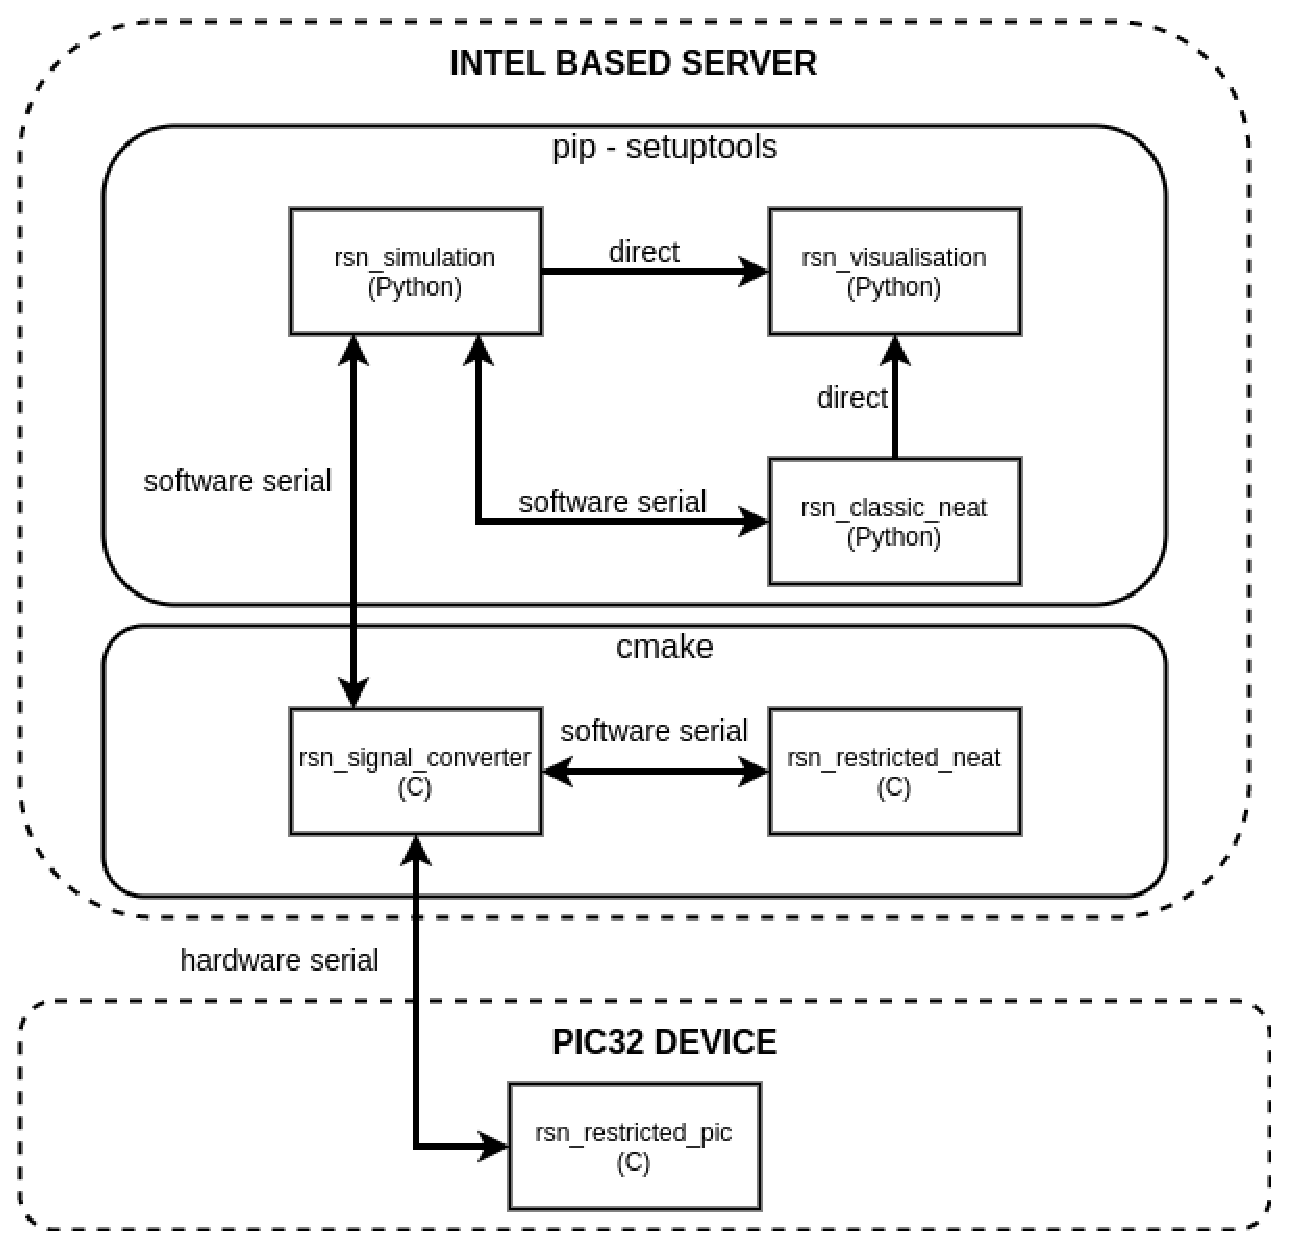
\includegraphics[width=0.6\textwidth]{figures/experiment_arch}
	\caption{The architecture of experimentation environment.}
	\label{fig:experiment_arch}
\end{figure}

%--------------------------------------------------------------------------------------------------
\FloatBarrier
\subsection{OpenAI Gym}

\FloatBarrier
\subsubsection{Cart pole}
A pole is attached by a non actuated joint to a cart, which moves along a frictionless track.
The system is controlled by applying a force of +1 or -1 to the cart.
The pendulum starts upright, and the goal is to prevent it from falling over. 
\begin{figure}[htb] 
	\centering
	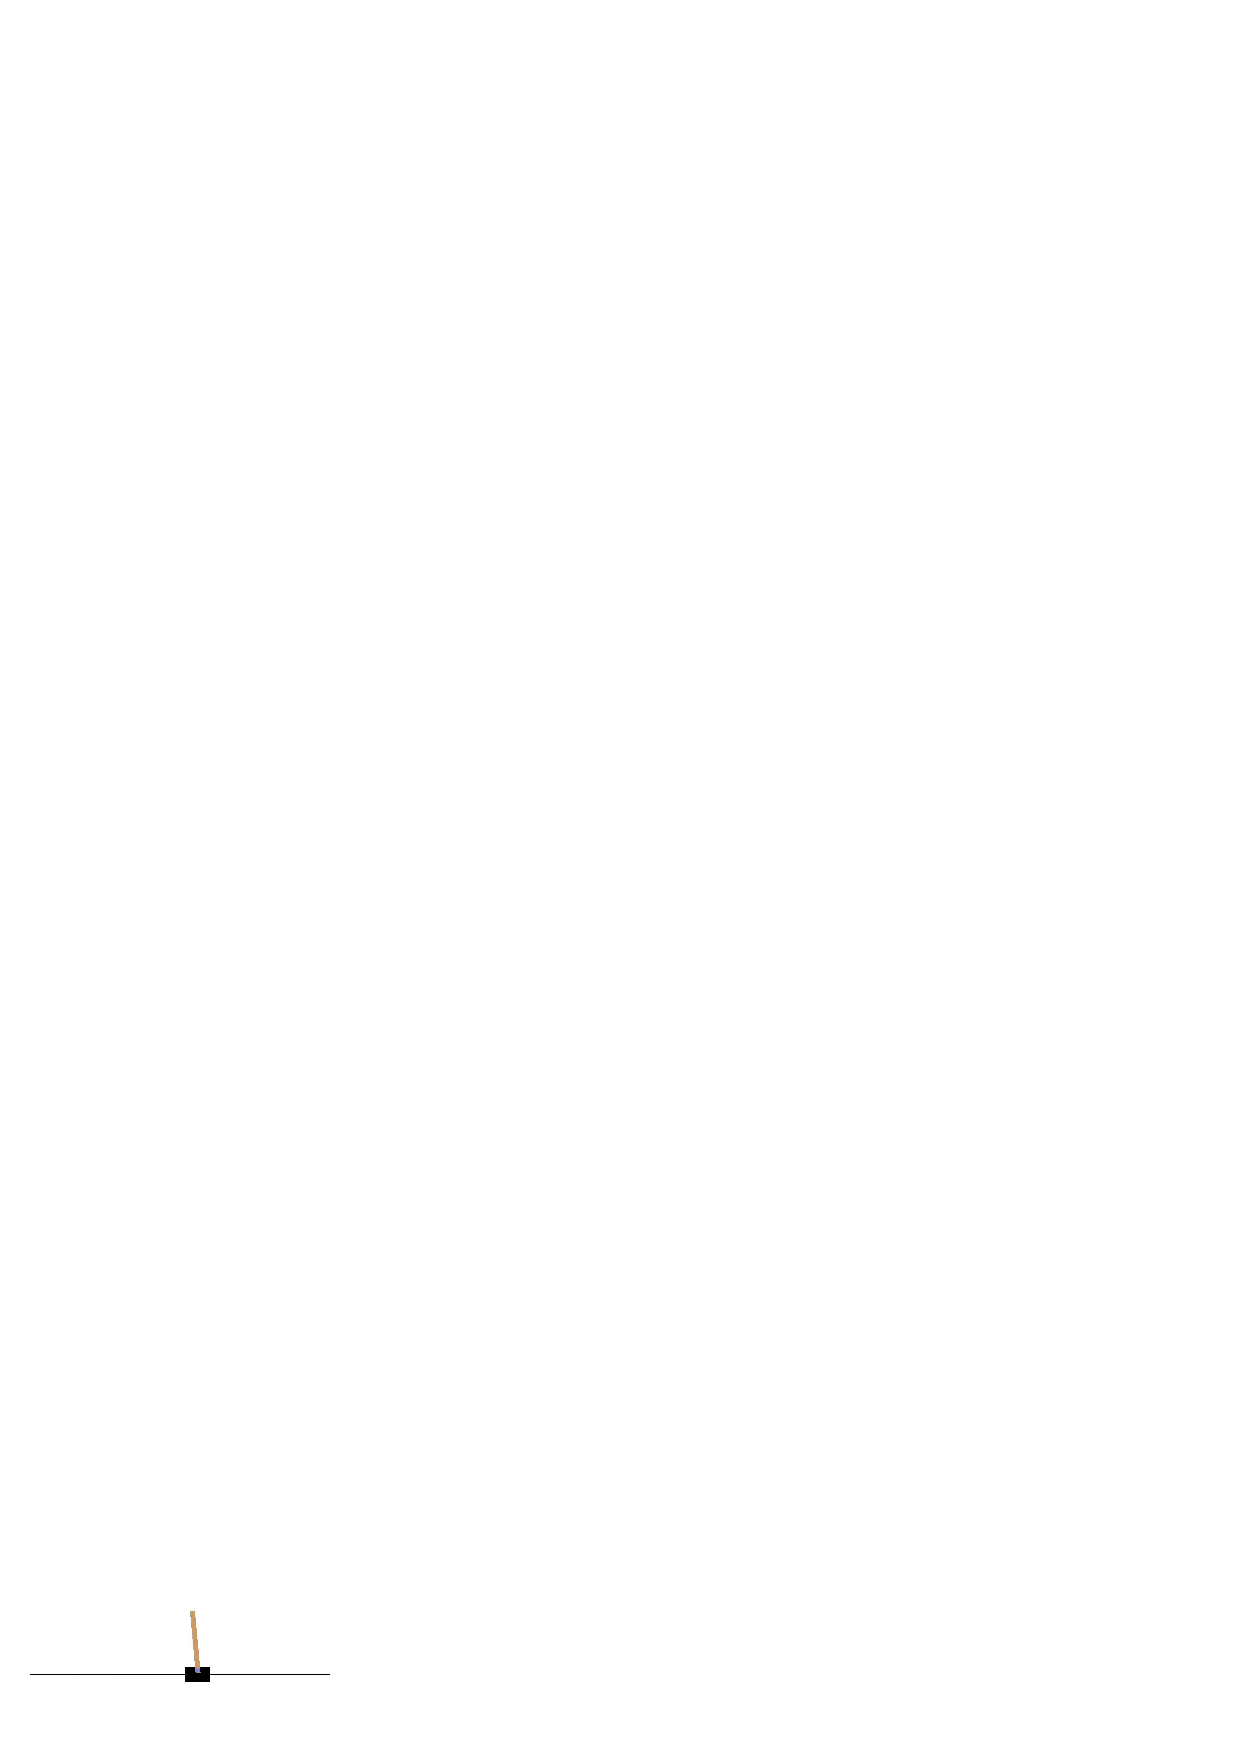
\includegraphics[width=0.6\textwidth]{figures/cartpole}
	\caption{A visualisation of cart pole environment.}
	\label{fig:cartpole}
\end{figure}
A reward of +1 is provided for every cycle that the pole remains upright.
The episode ends when the pole is more than 15 degrees from vertical, or the cart moves more 
than 2.4 units from the center.

\FloatBarrier
\subsubsection{Bipedal walker}
Reward is given for moving forward, total 300 points up to the far end. 
If the robot falls, it gets -100. Applying motor torque costs a small amount of points, 
more optimal agent will get better score.
State consists of hull angle speed, angular velocity, horizontal speed, vertical speed,
position of joints and joints angular speed, legs contact with ground, and 10 lidar 
rangefinder measurements
\begin{figure}[htb] 
	\centering
	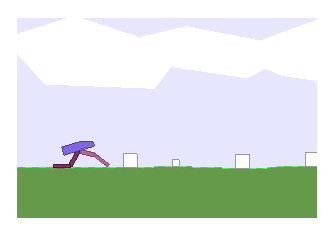
\includegraphics[width=0.6\textwidth]{figures/walker}
	\caption{A visualisation of walker environment in hardcore mode.}
	\label{fig:walker}
\end{figure}
Hardcore version adds ladders, stumps, pitfalls. Time limit is increased due to obstacles. 

\FloatBarrier
\subsubsection{Lunar lander}
Landing pad is always at coordinates (0,0). Coordinates are the first two numbers in state vector.
Reward for moving from the top of the screen to landing pad and zero speed 
is about 100..140 points.
If lander moves away from landing pad it loses reward back. Episode finishes if the lander 
crashes or comes to rest, receiving additional -100 or +100 points.
Each leg ground contact is +10. Firing main engine is -0.3 points each frame.
\begin{figure}[htb] 
	\centering
	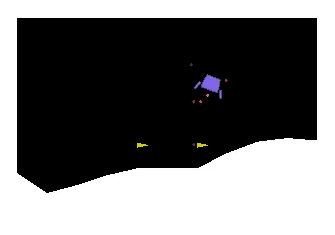
\includegraphics[width=0.6\textwidth]{figures/lunar}
	\caption{A visualisation of lunar lander environment.}
	\label{fig:lunar}
\end{figure}
Solved is 200 points. Landing outside landing pad is possible.
Fuel is infinite, so an agent can learn to fly and then land on its first attempt. 
Action is two real values vector from -1 to +1. First controls main engine, -1..0 off, 0..+1
throttle from 50\% to 100\% power. Engine can't work with less than 50\% power. 
Second value -1.0..-0.5 fire left engine, +0.5..+1.0 fire right engine, -0.5..0.5 off.

\FloatBarrier
\subsubsection{Robotank}
In this environment, the observation is an RGB image of the screen, which is an array of shape 
(210, 160, 3).

In Robotank, player is in control of a tank located in the middle of a barren field and must 
destroy enemy tanks after pinpointing their positions by using the window view and a small 
radar scope.

As shown on Figure \ref{fig:robotank}, game display is divided into two sections. 
The majority of the screen is occupied by the view of the battlefield, only objects in 
the front of vechicle are visible. 
The remainder of the screen consists of the status panel.

Located in the center of the status panel is a circular radar display with a sweeping arm.
If there is an enemy tank on the battlefield, it will appear on this display as a pink dot 
relative to robot position.
\begin{figure}[htb] 
	\centering
	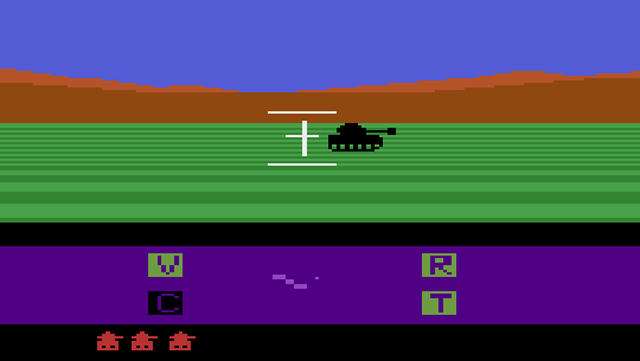
\includegraphics[width=\textwidth]{figures/robotank}
	\caption{A visualisation of robotank game frame that also serves as an input for network.}
	\label{fig:robotank}
\end{figure}

Situated around the radar display are four yellow boxes with capital letters in them.
These are the damage indicators. When your tank is shot, you suffer either a direct hit or a 
glancing shot. The first destroys your tank, the latter merely damages it.
The type of damage inflicted upon your tank is random.
If the V box is on, your video display will flash on and off. C means that your cannon 
firing power is cut in half. R indicates that your radar has been rendered useless.
T simply slows down the turning ability of your Robotank

%--------------------------------------------------------------------------------------------------
\FloatBarrier
\subsection{Computation device}

%==================================================================================================
\FloatBarrier
\section{Topological neural network implementation in low resource environment}

%--------------------------------------------------------------------------------------------------
\FloatBarrier
\subsection{Native implementation on 64-bit architecture}
Native representation of topologically varying neural network must rely on graph structure as 
simple matrix per layer representation assumes fully connected layered structure.
\begin{figure}[htb] 
	\centering
	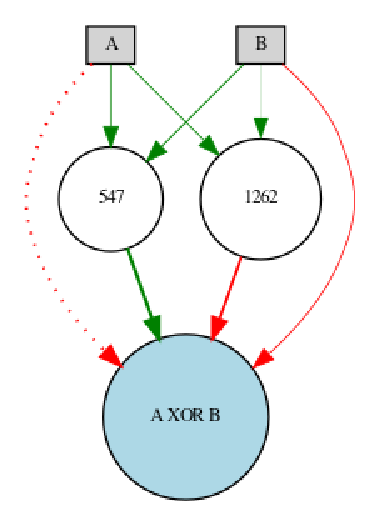
\includegraphics[width=0.3\textwidth]{figures/xor_network}
	\caption{An example of network graph for solving XOR problem.}
	\label{fig:xor_network}
\end{figure}
As shown on figure \ref{fig:xor_network} ANN consists of typical graph elements, 
nodes and links. Some of the nodes are recognised as an inputs or outputs where others are 
considered hidden nodes. While not visible on this visualisation nodes also need to store 
additional information, because of that a connection graph is also not a valid solution
as it only contains information about connection weights as shown on equation 
\ref{equ:connection_grid}.
\begin{equation}
	\label{equ:connection_grid}
	NET = \begin{bmatrix}
		0 & 0 & 2 & 2 & -1\\
		0 & 0 & 0 & 0 & 3\\
		0 & 0 & 0 & 0 & -3\\
	\end{bmatrix}
\end{equation}
Another significant disadventage is high memory requirements for use of that representation as 
each node requires its own row as well as column. This makes memory complexity of connection 
matrix $n^2$ where $n$ is number of nodes.
This negates one of main advantages of neuroevolution, it ability to create sparsly connected 
networks.
After rejecting that approach next logical step is selection of memory pointer functionality
that is natively implemented in most of lower level programming languages.
In shuch representation both nodes and links are stored in specialised structures in program
memory. Relations between those elements are modeled as a pointers to memory parts where target
objects are stored.
In case of solution described in this paper all implementation was done in C programming language
as it a solution with least overhead and a well established language in microcontroller
programming. 
Implementation details are crutial to thesis formed in this work an as such code listings will be
provided in a specific language instead of pseudocode.
\begin{lstlisting}[frame=single, language=C, caption={Implementation of Node and Link structures in C}]
typedef struct Node_t{
	int cycle;
	double value;
	double (*activation)(double);
	double (*agregation)(const Vector*);
	size_t connection_count;
	Connection** connections;
} Node;

typedef struct Connection_t{
	double weight;
	Node* target;
}Connection;
\end{lstlisting}
%--------------------------------------------------------------------------------------------------
\FloatBarrier
\subsection{Limitations in robotic applications}

%--------------------------------------------------------------------------------------------------
\FloatBarrier
\subsection{Computation efficiency - 24-bit fixed point model}

%--------------------------------------------------------------------------------------------------
\FloatBarrier
\subsection{Memory efficiency - offset based model}
